\subsubsection{Altidude Constante seguido de Arfagem}

Neste cenário, o objetivo é que o quadricóptero mantenha uma atitude fixa em arfagem (\textit{pitch}) enquanto estabiliza a altitude e as posições \(X\) e \(Y\). A análise considera a resposta dos controladores para cada uma dessas variáveis, observando-se as trajetórias real, estimada e de referência.

Parâmetros da simulação: \\

- Tempo total: 30 segundos;\\
- Altura desejada: 2 metros; \\
- Arfagem de 0.1 rad(5,73 graus) em t =5s

1) Arfagem

O gráfico a seguir mostra o comportamento do ângulo de arfagem ao longo do tempo.

\begin{figure}[H]
	\centering
	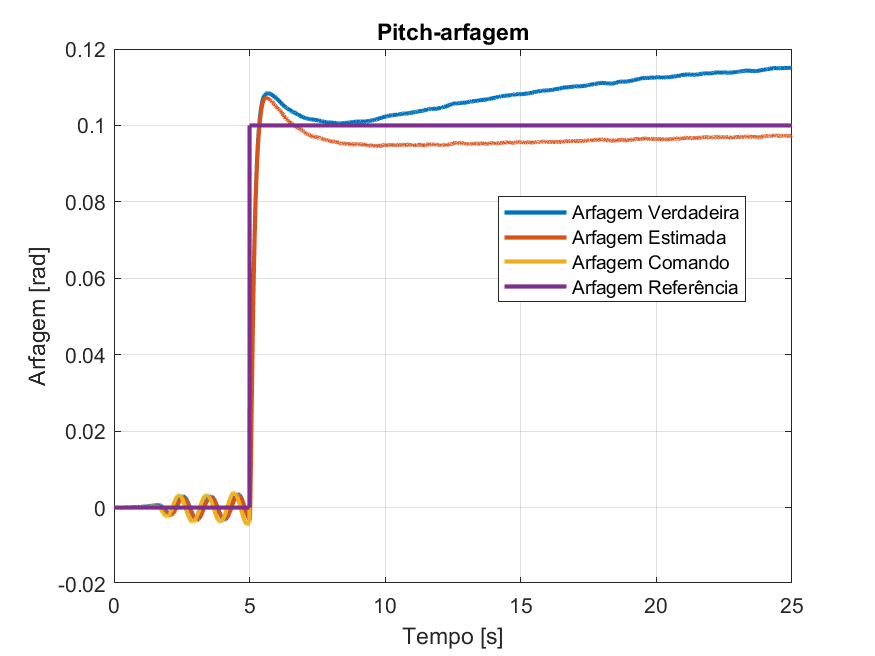
\includegraphics[width=0.8\textwidth]{Pitch-arfagem.png}
	\caption{Arfagem para o Cenário de Pitch}
	\label{fig:pitch-arfagem}
\end{figure}

Neste gráfico, observamos que o ângulo de arfagem responde rapidamente ao comando de referência, alcançando um valor de aproximadamente \(0.1\) radianos. Contudo, notamos uma pequena diferença entre a curva verdadeira (linha azul) e a estimada (linha laranja) após a arfagem. Essa diferença indica uma leve defasagem entre o valor verdadeiro e o valor estimado. A curva de referência (linha roxa) permanece constante, indicando o ângulo alvo desejado para este cenário.

2) Coordenada X

A seguir, temos o gráfico da posição \(X\) do quadricóptero ao longo do tempo.

\begin{figure}[H]
	\centering
	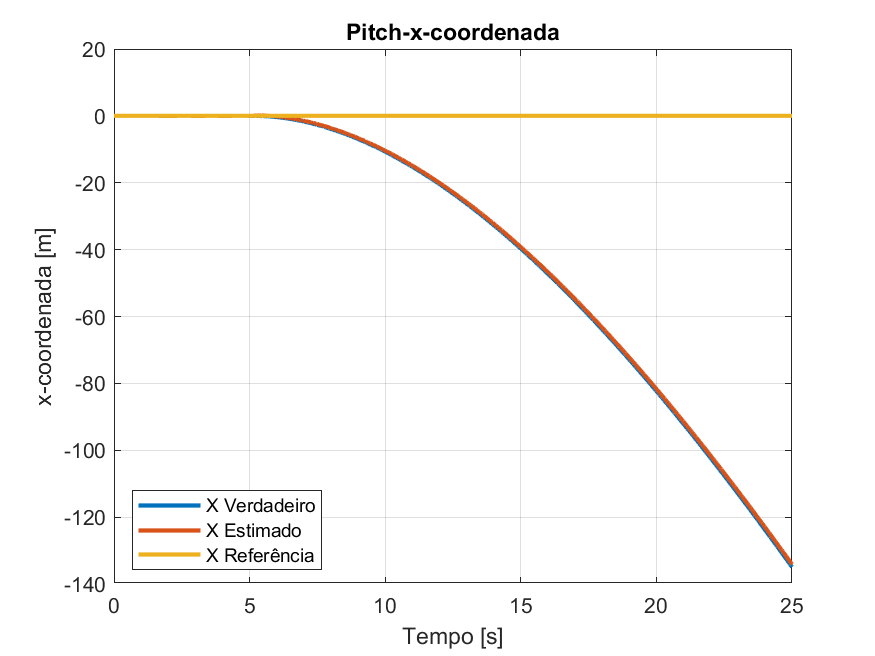
\includegraphics[width=0.8\textwidth]{Pitch-x-coordenada.png}
	\caption{Coordenada X para o Cenário de Pitch}
	\label{fig:pitch-x-coordenada}
\end{figure}

A posição \(X\) mostra um comportamento de translação contínua ao longo do tempo, conforme esperado para um cenário de arfagem constante, onde o quadricóptero se desloca em direção ao eixo \(X\). As curvas verdadeira e estimada (linhas azul e laranja) coincidem bem, indicando uma boa precisão na estimativa de posição.

3) Coordenada Z

Por fim, analisamos o comportamento da coordenada \(Z\) ao longo do tempo.

\begin{figure}[H]
	\centering
	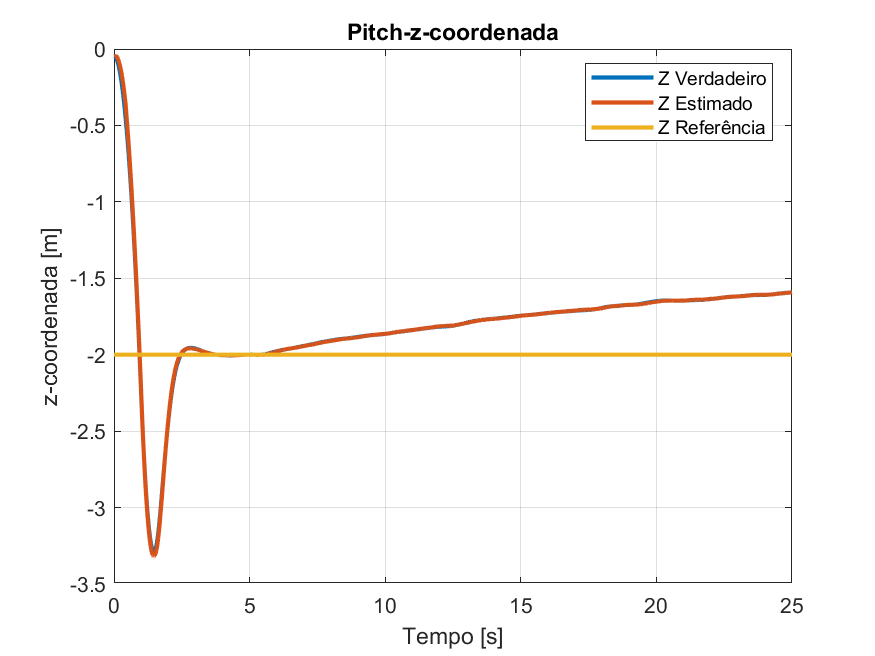
\includegraphics[width=0.8\textwidth]{Pitch-z-coordenada.png}
	\caption{Coordenada Z para o Cenário de Pitch}
	\label{fig:pitch-z-coordenada}
\end{figure}

Neste gráfico, a altitude mostra uma leve tendência de aumento com o passar do tempo, ainda que a referência de altura permaneça constante. A diferença entre as curvas verdadeira e estimada mostra que o sistema de controle está encontrando dificuldade para manter a altitude estável quando a inclinação de pitch é aplicada.

%### Conclusão Geral para o Cenário de Pitch

%O cenário de pitch revela um bom desempenho na estimativa de posição \(X\) e \(Y\), com ambas as curvas de posição verdadeira e estimada acompanhando bem a referência ao longo do tempo. No entanto, o controle de altitude apresenta uma leve instabilidade, o que pode exigir ajustes nos parâmetros do controlador para evitar desvios indesejados na coordenada \(Z\). Além disso, a leve diferença entre as curvas de arfagem verdadeira e estimada sugere que ajustes no controlador de pitch poderiam melhorar ainda mais a precisão da resposta do sistema.


%---------------------------------------------------------------------
% INDICE REMISSIVO
%---------------------------------------------------------------------
\phantompart
\printindex
%---------------------------------------------------------------------
